\section{Threat Modelling}

\textbf{Threat Modelling} consists in identifying threats in our system and then abstracting them into classes. This is done in order to find security issues and fix them as early as possible. In this case, we are going to study the \textbf{Precision Agriculture System}.

\subsection{Approach}

The first and most important step in Threat Modelling is to know what we want to protect and how we want to do it. There are two strategies from which we can choose: \textbf{Structured} and \textbf{Unstructured}. We are going to choose a Structured strategy, and, from the three Structured strategies available, we will be \textbf{Focusing on Assets}. We did so because we believe that this strategy is the one that will help us better understand what threats exist for this specific system. Alongside this strategy, we are going to use the \textbf{STRIDE} approach complemented with a \textbf{Data Flow Diagram}.

\subsubsection{Focusing on Assets}

When we are Focusing on Assets while searching for potential threats in our system, it is important to think about 3 topics: \textbf{Things attackers want}, \textbf{Things you want to protect}, and \textbf{Stepping stones to either of these.} Considering our Agriculture System, we answered these topics:

\textbf{Things attackers want}
\begin{itemize}
  \item User passwords
  \item System Knowledge
  \item Information about crops/plantations (Field Data)
  \item Disrupt/sabotage production
\end{itemize}

\textbf{Things you want to protect}
\begin{itemize}
  \item Valuable Information (Passwords/System Knowledge/Field Data)
  \item Fields (Prevent any kind of sabotage)
  \item Company Reputation
\end{itemize}

\textbf{Stepping stones to either of these}
\begin{itemize}
  \item Authentication System
  \item Firewall
  \item Secure Communication Channels
\end{itemize}



\subsection{System Modelling}

In order to better understand a complex system, it is useful to represent it with the help of diagrams. In this case we represented our systems through a \textbf{Data Flow Diagram}.

In order to create the diagram we need to dissect our system to make it simpler. The \textbf{precision agriculture system} consists in a series of integrated \textbf{sensors} that gather data such as temperature and humidity, sending it via a wireless interface to a \textbf{base station/gateway}. One farm may have up to a thousand sensors. There are also \textbf{actuators} that control watering systems or greenhouse temperatures. The next component of our systems are the \textbf{gateways}. These communicate with several sensors/actuators via radio interfaces, adjusting their operation according to analytics provided by the \textbf{backend}. Our \textbf{cloud-based backend} is responsible for storing data and for all analytics in our system. It also sends new application rules back to the gateways. At last, we also have a \textbf{Dashboard/GUI} so that Farmers and Experts can interact with the system.

 \begin{figure}[ht!]
 	\centering
 	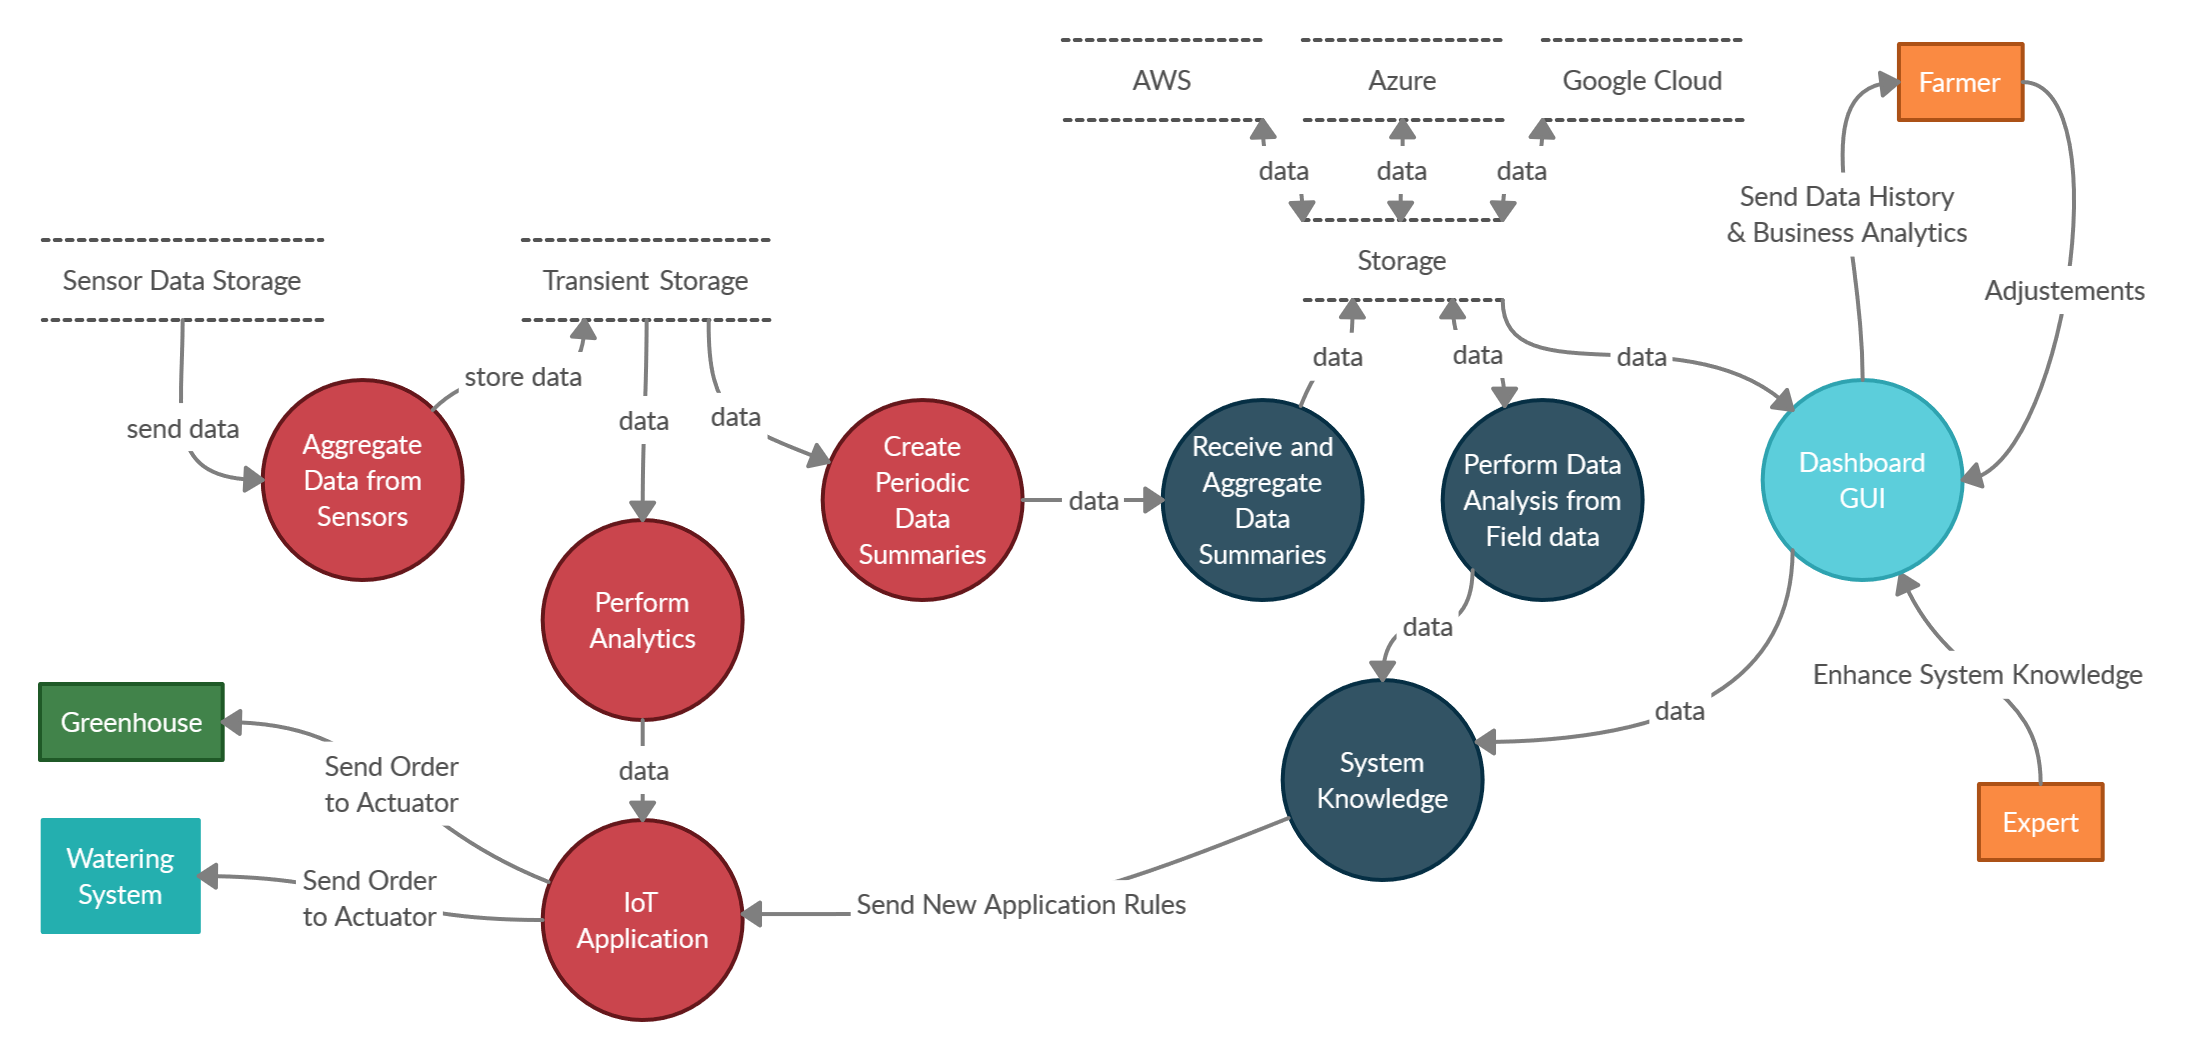
\includegraphics[width=1\linewidth]{img/dfd.png}
 	\caption{Data Flow Diagram}
 \end{figure}
 
 To create this diagram we sorted all elements of our system by their respective category: \textbf{processes}, \textbf{data flows}, \textbf{data stores} and \textbf{external entities}. Starting by our processes, we considered all running code in our system as a process, using different colors to identify to which module they belong: \textbf{red} processes belong to the \textbf{gateways}, \textbf{dark blue} processes belong to the \textbf{backend} and \textbf{light blue} processes belong to the \textbf{Dashboard/GUI}. Since we didn't consider \textbf{sensors} to be external entities, we represented them as \textbf{data stores}. We did this because the sensors are the most atomic element of this system, and their only purpose is to gather data and then forward it to their respective gateway. In contrast, we considered elements such as \textbf{Watering Systems} and \textbf{Greenhouses} to be external entities, since our system's actuators perform actions on them, but they aren't part of the system itself. Another decision we made, was to consider our cloud based storage providers as data stores, and not external entities. This decision was made because their only purpose is to provide cloud storage. They wont interact with our backend in other ways.

\subsection{Finding Threats}

After dissecting our system in smaller parts, we made it much more simple to see what can or cant go wrong during it's operation. Also, we were given some general security requirements that we need to include: Integrity, Authentication, Availability, Auditing and Privacy and Anonymity. 
In order to find the relevant threats, we will be using the STRIDE methodology. To make it simple to understand which element has a certain threat, we will be grouping them by elements.

\subsubsection{STRIDE}

\paragraph{Sensors \& Actuators}\mbox{}

\textbf{Spoofing}

\begin{itemize}
    \item An attacker could setup a connection with a malicious gateway and instruct actuators to execute orders that might hurt the production such as overheating a greenhouse or never turning off the watering system. This might be addressed with the use of public key authentication on these communication channels.
\end{itemize}

\textbf{Tampering}

\begin{itemize}
    \item An attacker (or a faulty sensor) could send wrong or misleading data to a gateway. This can compromise the integrity of our data. The amount of sensors in our system may lead to these kind of problems being more or less severe. One possible fix would be to identify sensor (with a secure and unique id) by regions/sections of a farm, and having a larger amount of them. With this, we are able to know if we are handling a faulty sensor or some kind of attack.
\end{itemize}

\textbf{Repudiation}
\begin{itemize}
    \item The lack of proper authentication doesn't allow us to guarantee that we can associate an order given to an actuator to the respective gateway that gave the order. This can also be fixed by implementing proper authentication.
\end{itemize}

\textbf{Information Disclosure}

\begin{itemize}
    \item The actuators are vulnerable to Information Disclosure since the communication channels do not provide any kind of authentication as we have seen. We can solve this by also using public key authentication.
\end{itemize}

\textbf{Denial of Service}
\begin{itemize}
    \item The actuators have weak processors, so its easy to fill the communication interface with fake orders, this will make them struggle to operate correctly and modify the state of the farm devices.
\end{itemize}

\textbf{Elevation of Privilege}
\begin{itemize}
    \item Since the sensors can be devices like Raspberry devices and similar, there is a big chance of an attacker being able to run code remotely on them.
\end{itemize}

\paragraph{Basestation/Gateway}\mbox{}

\textbf{Spoofing}

\begin{itemize}
    \item An attacker could setup fake nodes and actuators and feed false information to the gateways. As we have seen before, this can be fixed with the use of public key authentication on these communication channels.
\end{itemize}

\textbf{Tampering}

\begin{itemize}
    \item An attacker could modify the transient storage of a certain gateway, affecting the integrity of the data collected. This can be avoided by encrypting the data aggregated from the sensors.
\end{itemize}

\textbf{Repudiation}
\begin{itemize}
    \item The lack of proper authentication doesn't allow us to guarantee that we can associate data received from sensors to the respective sensor. The IoT application also has no way of knowing that new Application Rules come from the legitimate backend. This can also be fixed by implementing proper authentication.
\end{itemize}

\textbf{Information Disclosure}

\begin{itemize}
    \item With an attack focused in the transient storage, it is possible to get some critical data about the system. Making it easier for the attacker to execute stronger attacks in the future.
\end{itemize}

\textbf{Denial of Service}

\begin{itemize}
    \item The lack of authentication allows an attacker to send false data to a gateway. If an attackers repeatedly sends information to the gateway, the transient storage may fill up and render the gateway useless. By sending a large amount of "fake" sensor data, an attacker may also disrupt the reception of data from actual sensors. As seen before, authentication may be used to solve this by discarding harmful connections.
\end{itemize}

\paragraph{Cloud Back-End}\mbox{}

\textbf{Spoofing}

\begin{itemize}
    \item The lack of an authentication system allows an attacker to pose as a gateway of our system. This can be solved the same way as before.
\end{itemize}

\textbf{Tampering}

\begin{itemize}
    \item The lack of an authentication system allows an attacker to feed false data summaries to our backend, compromising the integrity of our data. This can be solved the same way as before.
\end{itemize}

\textbf{Repudiation}
\begin{itemize}
    \item The backend receives data summaries and stores them in the cloud, but there is no way to know from which gateway they come. This could be solved by including any kind of identification inside the summaries and by using a secure communication protocol.
\end{itemize}

\textbf{Information Disclosure}
\begin{itemize}
    \item The backend uses cloud storage which itself may have security issues or access data without our permission. Also, we need to assure that the connection between the backend and cloud storage is secure.
\end{itemize}

\textbf{Denial of Service}

\begin{itemize}
    \item An attacker sending false data summaries can overload the backend's capability of processing other summaries, and, in extreme fill up our cloud storage. As seen before, authentication may be used to solve this by discarding harmful connections.
\end{itemize}

\textbf{Elevation of Privilege}

\begin{itemize}
    \item If the content of the received data summaries is not checked for incorrect or harmful content, an attacker could run commands or modify data on our backend. This could be resolved by implementing a module for content scan.
\end{itemize}

\paragraph{Dashboard/GUI}\mbox{}

\textbf{Spoofing}

\begin{itemize}
    \item In order to avoid that attackers pose as users (farmers) or experts, we need to implement a login system to avoid unwanted access.
\end{itemize}

\textbf{Repudiation}

\begin{itemize}
    \item In order to know that a certain user is indeed a farmer or expert, we need to implement a login system so that we can associate a session to a user.
\end{itemize}

\textbf{Denial of Service}

\begin{itemize}
    \item If there is no mechanism of detecting these kind of attacks, an attacker could, for example, create a bot to flood our Dashboard/GUI with login requests, interrupting real users to access the system.
\end{itemize}

\textbf{Elevation of Privilege}

\begin{itemize}
    \item If there is input validation, an attacker may be able to execute unwanted code. This may be fixed may validating input.
\end{itemize}


\paragraph{Summary of Threats}\mbox{}

In the following table we made a \textbf{Summary of Threats} of our system, using the numbers 1 to 4 to represent each of our elements: 1 - Sensors \& Actuators, 2 - Basestation/Gateway, 3 - Cloud Back-End, and 4 - Dashboard/GUI. This summary helps us understand which threats each element is exposed to.

\begin{table}[h!]
\centering
 \begin{tabular}{|l|c|c|c|c|} 
 \hline
 \textbf{Threat} & 1 & 2 & 3 & 4 \\
 \hline
 \textbf{S}poofing & X & X & X & X \\ 
 \hline
 \textbf{T}ampering & X & X & X & - \\
 \hline
 \textbf{R}epudiation & X & X & X & X \\
 \hline
 \textbf{I}nformation Disclosure & X & X & X & - \\
 \hline
 \textbf{D}enial-of-Service & X & X & X & X \\
 \hline
 \textbf{E}levation of Privilege & X & - & X & X \\
 \hline
 \end{tabular}
\end{table}

% Passos por alto
% escolher a estratégia estrutura FOCUSING ON ATTACKERS ou ASSETS
% seguir o four step framework
    % System Modelling -> fazer um dfd do sistema
    % analisar cada um dos 4 modulos individualmente e dps juntar td (dica do professor)
    
    % encontrar as ameaças 
        % stride
        % fazer a tabela como tem nos slides era porreiro
        
    